\documentclass[xcolor=pdflatex,dvipsnames,table]{beamer}
\usepackage{algorithmic}
\usepackage{multimedia}

\usepackage[absolute,overlay]{textpos} 


\newcommand\putpic[5]{% 
        \begin{textblock}{#3}(#1,#2) 
  \includegraphics[width=#3\TPHorizModule, 
  height=#4\TPVertModule]{#5} 
     \end{textblock} 
} 

\newcommand\putmov[5]{% 
        \begin{textblock}{#3}(#1,#2) 
  \movie[width=#3\TPHorizModule, 
  height=#4\TPVertModule]{#5} 
     \end{textblock} 
} 

\usetheme{default}



\setbeamercolor{umbcboxes}{bg=violet!12,fg=black}

\usepackage{rotating} % for defining \schwa
\newcommand{\schwa}{\raisebox{1ex}{\begin{turn}{180}e\end{turn}}}

\newcommand{\arcsinh}{\mathop\mathrm{arcsinh}\nolimits}
\newcommand{\arccosh}{\mathop\mathrm{arccosh}\nolimits}
\newcommand{\Pu}{P_{\mathrm{amb}}}

\title{Path-Selection in Floating Sensor Networks}
\author[K. Weekly]{Kevin Weekly}
\institute[UCB]{
  Dept. of Electrical Engineering and Computer Sciences\\
  University of California, Berkeley \\
}
\date{April 15, 2011}

\begin{document}

\begin{frame}[plain]
  \titlepage
\end{frame}

%%%%%%%%%%%%%%%%%%%%% INTRODUCTION %%%%%%%%%%%%%%%%%%%%%%%%%%%%%%%%%%%%%%%%%%%%%%%%%%%%%%%
\section{Introduction}
\begin{frame}{Introduction to the Floating Sensor Network}
\begin{columns}
\column{0.5\linewidth}
\begin{itemize}
\item Motorized lagrangian (non-anchored) sensors to map currents in rivers and estuaries.
\item Fleet of 40 to deployed in Summer 2011, running experiments in multi-vehicle coordination.
\item Fleet must respond within minutes to changing river conditions or user objectives.
\item IPs provide powerful tool to obtain \emph{optimal} strategies for the fleet to maximize its utility.
\end{itemize}

\column{0.5\linewidth}
\begin{figure}
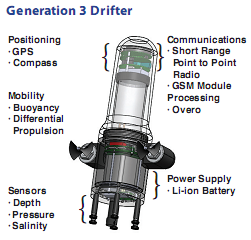
\includegraphics[height=0.5\textheight]{figures/drifter.png}\\
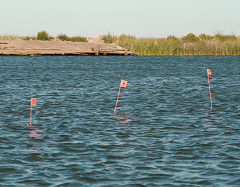
\includegraphics[width=1\textwidth,height=0.3\textheight,clip,trim=0 20 0 20,keepaspectratio=true]{figures/drifter_in_water.png}
\end{figure}
\end{columns}
\end{frame}


%% We want first outline to come after introduction slide
\AtBeginSection[]
{
   \begin{frame}
       \tableofcontents[currentsection]
   \end{frame}
}

%%%%%%%%%%%%%%%%%%%%% LINK LABELLING %%%%%%%%%%%%%%%%%%%%%%%%%%%%%%%%%%%%%%%%%%%%%%%%%%%%%%%
\section{Problem Setup}
\subsection{Software}
\begin{frame}[fragile]{Problem Setup: Software}
\begin{columns}
\column{0.5\linewidth}
\small
OpenOpt: Python package to construct problems for variety of solvers (we use cplex and glpk)
{\footnotesize
\begin{verbatim} # Instantiate min(f * x) s.t. Ax >= b
# x_i are integer, where i in intVars
p = MILP(f=f, lb=lb, ub=ub, A=A, b=b,
    intVars=intVars, goal='max')

# Start the solver : 'cplex' or 'glpk'
r = p.solve('cplex') \end{verbatim}
}
\begin{itemize}
\item Integrates with our python-based drifter architecture.
\item Python file \& image libraries immediately available to set-up problem.
\end{itemize}

\column{0.5\linewidth}
\begin{figure}

\includegraphics[width=0.8\textwidth]{figures/python.png}\\
$\downarrow$\\

\includegraphics[width=0.8\textwidth]{figures/openopt.png}\\
$\downarrow$\\

\includegraphics[width=0.4\textwidth]{figures/cplex.png}

\includegraphics[width=0.4\textwidth]{figures/gnu-head-sm.jpg}
\end{figure}
\end{columns}
\end{frame}

\subsection{Link Labelling}
\begin{frame}{Problem Setup: Link Labelling}
Breadth-First-Search (BFS) style flood-fill:
\begin{itemize}
   \item Maintains edge list of water pixels to process and processes them in BFS order.
   \item Each edge is given a label. As it sweeps through the domain, that label is assigned to underlying pixels.
   \item Monitors continuity of edges.
\begin{itemize}
    \item Path Splitting: If a previously continuous edge becomes broken, two new labels are generated and connections are recorded. 
    \item Path Joining: If two edges meet, a new label is generated and connections are recorded.
\end{itemize}
   \item Algorithm ends when there are no more water pixels to process.
\end{itemize}
\end{frame}

\begin{frame}{Problem Setup: Link Labelling}
\begin{columns}[c]
\column{0.5\linewidth}
San Joaquin/Sacramento River Delta Target Domain
\begin{itemize}
 \item Approx. 2km$\times$8km 
 \item 105 labelled regions after pruning 0-area regions
\end{itemize}

Weaknesses:
\begin{itemize}
 \item ``King's move'' dynamics.
 \item Bias towards coordinate system.
 \item Several long strips.
 \item Joining of labels relies on timing.
\end{itemize}


\column{0.5\linewidth}
  \begin{figure}
  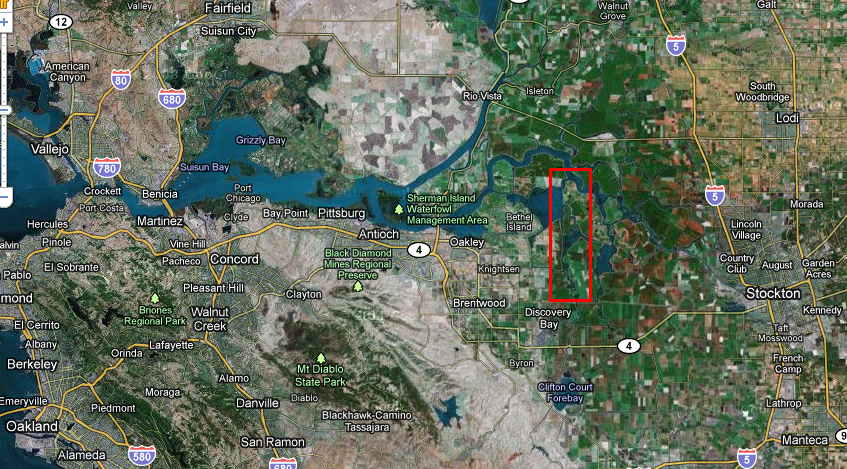
\includegraphics[width=1\linewidth]{figures/domain.png}\\
  \movie[width=0.5\linewidth, height=0.5\textheight, rate=2, autostart, autoplay, repeat, poster]{}{figures/anim.flv}
  \hfill
  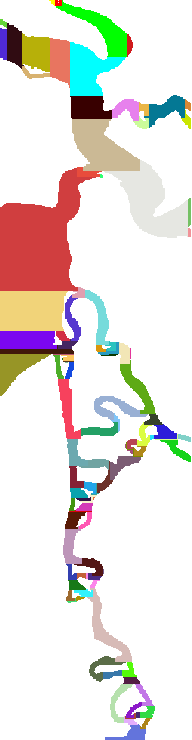
\includegraphics[height=0.5\textheight]{figures/labelled.png}
  \end{figure}
\end{columns}
\end{frame}


%%%%%%%%%%%%%%%%%%%%% PATH ENUMERATION %%%%%%%%%%%%%%%%%%%%%%%%%%%%%%%%%%%%%%%%%%%%%%%%%%%%%%%
\subsection{Path Enumeration}
\begin{frame}{Problem Setup: Path Enumeration}
\begin{columns}
 \small
 \column{0.5\linewidth}
Depth-First-Search (DFS) through connection list:
\begin{itemize}
 \item Exhaustively enumerates all possible paths to predetermined ``sink'' labels.
 \item Connections are directed based on order they were encountered during labelling-- a path cannot backtrack.
 \item If a dead-end is reached, DFS attempts to ``punch-through'' a connection directed against it (that was not already visited).
\end{itemize}

 \column{0.5\linewidth}
\begin{tabular}{c|l}
 \movie[width=0.5\linewidth, height=0.8\textheight, rate=1, autostart, autoplay, repeat, poster]{}{figures/paths.flv} &
 \small {1547 paths found}
\end{tabular}

\end{columns}

\end{frame}

%%%%%%%%%%%%%%%%%%%%% STATIC FORMULATION %%%%%%%%%%%%%%%%%%%%%%%%%%%%%%%%%%%%%%%%%%%%%%%%%%%%%%%
\section{\{0,1\} Static Linear Programs}
\subsection{Formulation}
\begin{frame}{\{0,1\} Static Linear Programs: Formulation}
\begin{align*}
\max_{x,y}\;& -g^Tx + h^Ty \\
\mbox{s.t.}\;& \left[ \begin{array}{c}
                       A\\
                       -1, \dots, -1
                      \end{array}\right] x \geq \left[ \begin{array}{c} y\\-D \end{array}\right] \\
&a_{ij} = \begin{cases}
           1\;\mbox{if path $i$ contains link $j$}\\
           0\;\mbox{otherwise}
          \end{cases}\\
&x_i \in \{0,1\}\;\forall i\in\{1\dots n\}\\
&y_j \in \{0,1\}\;\forall j\in\{1\dots m\}
\end{align*}

\begin{itemize}
\item $\{x_i\}$ : indicates whether path $i$ of $n$ total paths is taken.
\item $\{y_j\}$ : indicates whether link $j$ of $m$ total links is visited.
\item $D$ : total number of units avaiable.
\item Preprocessing step : Remove all links impossible to visit (zero-rows of A).
\end{itemize}

\end{frame}


%%%%%%%%%%%%%%%%%%%%%% ALL LINKS MINIMUM UNITS %%%%%%%%%%%%%%%%%%%%%%%%%%%%%%%%%%%%%%%%%%%%%%
\subsection{All links minimum units}
\begin{frame}{\{0,1\} Static Linear Programs: All links minimum units}
\emph{``Visit every link using the least number of drifters''}
\begin{align*}
g &= \left[ 1,1, \dots ,1\right]\\
y &= \left[ 1,1, \dots ,1\right]\\
D &= \infty \;\mbox{(remove row from ILP)}
\end{align*}

\begin{itemize}
 \item Preprocessing : Find paths which must be taken ( rows of A containing only one 1 ). Remove these paths and all of their links from ILP. Repeat until all rows of A have two or more 1s.
\end{itemize}
\end{frame}

\begin{frame}{\{0,1\} Static Linear Programs: All links minimum units}
\begin{figure}
\rowcolors{1}{RoyalBlue!20}{RoyalBlue!5}
  \begin{tabular}{|l|c|}
  \hline 
  Paths in ILP/Total & 1544/1547 \\
  Labels in ILP/Total & 70/105 \\
  CPU Time (cplex) & 250mS\\
  CPU Time (glpk) & 180mS \\
  Units Needed & 10 \\
  \hline
  \end{tabular}
\end{figure}

  \begin{figure}
     {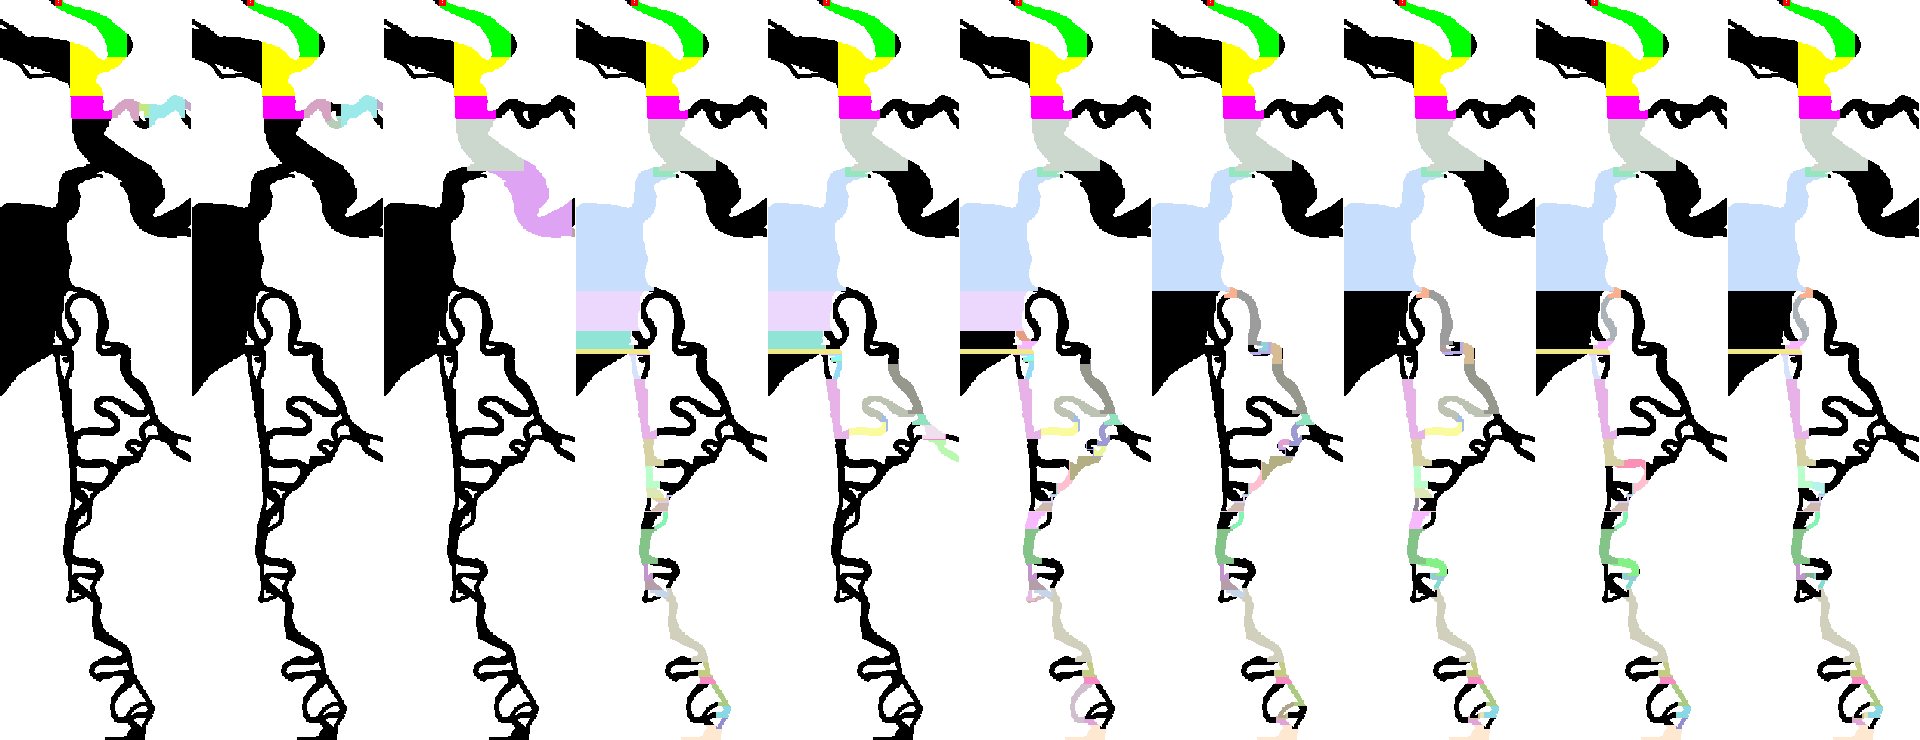
\includegraphics[width=1\textwidth]{figures/all_links_minimum_units_paths.png}}
  \end{figure}
\end{frame}


%%%%%%%%%%%%%%%%%%%%%% MAX COVERAGE FIXED UNITS %%%%%%%%%%%%%%%%%%%%%%%%%%%%%%%%%%%%%%%%%%%%%
\subsection{Max coverage fixed units}
\begin{frame}{\{0,1\} Static Linear Programs: Max coverage fixed units}
\emph{``Visit the greatest total weighted area with a fixed number of units.''}
\begin{align*}
g &= 0\\
h &= \left[ w_1,w_2, \dots ,w_m\right]\\
D &= 5\\
\end{align*}

\begin{itemize}
 \item Path processing : Set $w_j$ to the weight of each region with label $j$.
 \item Note: Setting $w_j=1$ solves the problem\\ \emph{``Visit the most number of links with a fixed number of units.''}
\end{itemize}
\end{frame}

\begin{frame}{\{0,1\} Static Linear Programs: Max coverage fixed units}
Example: $w_j$ are the number of pixels in each region.
\begin{figure}
\rowcolors{1}{RoyalBlue!20}{RoyalBlue!5}
  \begin{tabular}{|l|c|}
  \hline 
  Paths & 1547 \\
  Labels in ILP/Total & 82/105 \\
  CPU Time (cplex) & 440mS\\
  CPU Time (glpk) & 210mS \\
  Allotted Units & 5\\
  Pixels covered/Total & 31169/32033 (97\%)\\
  \hline
  \end{tabular}
\end{figure}

  \begin{figure}
     {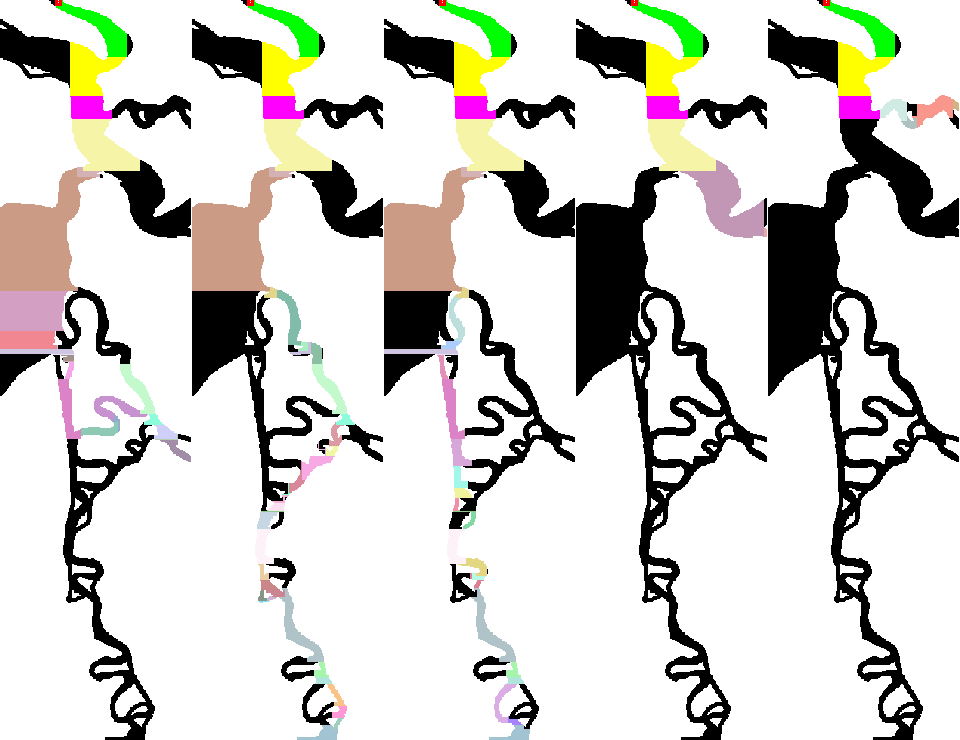
\includegraphics[width=0.5\textwidth]{figures/max_coverage_fixed_units_paths.png}}
  \end{figure}
\end{frame}

%%%%%%%%%%%%%%%%%%%%% DYNAMIC FORMULATION %%%%%%%%%%%%%%%%%%%%%%%%%%%%%%%%%%%%%%%%%%%%%%%%%%%%%%%

\section{\{0,1\} Dynamic Linear Programs}
\subsection{Formulation}
\begin{frame}{\{0,1\} Dynamic Linear Programs: Formulation}
\begin{align*}
\max_{x,y}\;& -g^T \tilde{x} + h^T \tilde{y} \\
\mbox{s.t.}\;& \left[ \begin{array}{c}
                       \tilde{A}\\
                       -1, \dots, -1
                      \end{array}\right] \tilde{x} \geq \left[ \begin{array}{c} \tilde{y}\\-D \end{array}\right] \\
&a_{i,\mbox{\tiny map}(j,t)} = \begin{cases}
           1\;\mbox{if path $i$ passes link $j$ at time $t$}\\
           0\;\mbox{otherwise}
          \end{cases}\\
&\tilde{x}_i \in \{0,1\}\;\forall i\in\{1\dots \tilde{n}\}\\
&\tilde{y}_{\mbox{\tiny map}(j,t)} \in \{0,1\}\;\forall j\in\{1\dots m\},t\in\{1\dots T\}
\end{align*}

\begin{enumerate}
\small
\item Set the time-horizon, $T$, to the maximum path length.
\item Enumerate all paths which can delay at the source node and still arrive at a sink node by $T$. 
\item $\tilde{x}$ now contains original $x$ plus all ``delayed'' paths.
\item $\tilde{y}$ indicates which links are visited and \emph{when}.
\item Preprocessing step : Remove all zero-rows of A.
\end{enumerate}
\end{frame}

%%%%%%%%%%%%%%%%%%%%% ALL TIME ALL PATHS MINIMUM UNITS %%%%%%%%%%%%%%%%%%%%%%%%%%%%%%%%%%%%%%%%%%%%%%%%%%%%%%%
\subsection{All time all links minimum units}
\begin{frame}{\{0,1\} Dynamic Linear Programs: All time all links minimum units}
\begin{columns}

\column{0.5\linewidth}
  \emph{``Within the time it takes to traverse the entire domain, maintain observation of as many regions as feasibly possible, using the minimum number of units. Units may only delay at the drop-off or pick-up points.''}
  \begin{figure}
  \rowcolors{1}{RoyalBlue!20}{RoyalBlue!5}
    \begin{tabular}{|l|c|}
    \hline 
    Paths in ILP/Total & 17328/17487 \\
    Labels in ILP/Total & 1308/4935 \\
    CPU Time (problem setup) & 50s \\
    CPU Time (cplex) & 5s \\
    CPU Time (glpk) & 128s \\
    Time Horizon & 47 steps\\
    Units Needed & 311 \\
    \hline
    \end{tabular}
  \end{figure}


\column{0.5\linewidth}
  \begin{figure}
    \centering
    \hfill
    \movie[width=0.5\linewidth, height=0.7\textheight, rate=2, autostart, autoplay, repeat, poster]{}{figures/all_time_all_links_min_units.flv}
  \end{figure}

\end{columns}
\end{frame}

%%%%%%%%%%%%%%%%%%%%% ALL TIME MAX COVERAGE FIXED UNITS %%%%%%%%%%%%%%%%%%%%%%%%%%%%%%%%%%%%%%%%%%%%%%%%%%%%%%%
\subsection{All time max coverage fixed units}
\begin{frame}{\{0,1\} Dynamic Linear Programs: All time max coverage fixed units}
\begin{columns}

\column{0.5\linewidth}
  \emph{``Over the time it takes to traverse the entire domain, maximize the total area observed given a fixed number of units. Units may only delay at the drop-off or pick-up points.''}
  \begin{figure}
  \rowcolors{1}{RoyalBlue!20}{RoyalBlue!5}
    \begin{tabular}{|l|c|}
    \hline 
    Paths in ILP & 17487 \\
    Labels in ILP/Total & 2028/4935 \\
    CPU Time (problem setup) & 51s \\
    CPU Time (cplex) & 8s \\
    CPU Time (glpk) & 6s \\
    Time Horizon & 47 steps\\
    Units Allotted & 40\\
    Pixels Covered/Total & 71k/99k (72\%)\\
    \hline
    \end{tabular}
  \end{figure}


\column{0.5\linewidth}
  \begin{figure}
    \centering
    \hfill
    \movie[width=0.5\linewidth, height=0.7\textheight, rate=2, autostart, autoplay, repeat, poster]{}{figures/all_time_max_coverage_fixed_units.flv}
  \end{figure}
\end{columns}
\end{frame}

%%%%%%%%%%%%%%%%%%%%% FULL-SCALE OPERATION %%%%%%%%%%%%%%%%%%%%%%%%%%%%%%%%%%%%%%%%%%%%%%%%%%%%%%%
\section{Full scale operation example}
\begin{frame}{Full scale operation example: Motivation}
\begin{columns}
\column{0.5\linewidth}
\begin{itemize}
 \small
 \item Units cannot travel upstream, only choose which branch of the river to flow down. 
 \item Units can stop themselves by running into the shore, but will not be able to continue without rescue. 
 \item Boats periodically \emph{extract} units which have reached the downstream edge of the domain and re-\emph{insert} them back at the upstream edge.
 \item Boats have finite speed and thus can only re-insert units a fixed number of times throughout the experiment.
\end{itemize}


\column{0.5\linewidth}
 \begin{figure}
     {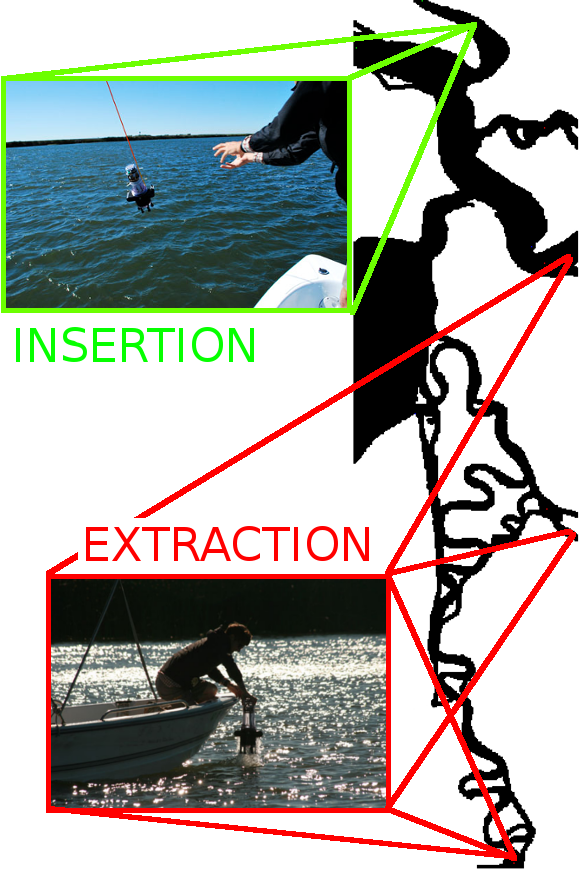
\includegraphics[height=.8\textheight]{figures/full_scale.png}}
  \end{figure}
\end{columns}
\end{frame}

\begin{frame}{Full scale operation example: Formulation}
\small
\begin{itemize}
 \item Objective function same as ``All time max coverage fixed units.''
 \item Time divided into discrete \emph{deployment windows} representing twice the transit time of a boat. 
 \item The number of paths which can start at the beginning of a window is the amount of paths terminating at least one transit time previously.
 \item Constraint on total number of drifters replaced with:
\begin{align*}
  \left[\begin{array}{ccccccccc}
   1&\dots&1&0&\dots&0&0&\dots&0\\
   0&\dots&0&1&\dots&1&0&\dots&0\\
   &&&&\vdots&&&&
  \end{array}\right] \tilde{x} \leq R \tilde{x} + \left[\begin{array}{c}D\\0\\\vdots\\0\end{array}\right]\\
 R_{i\mbox{\tiny map}(j,d)} = \begin{cases}
				1\;\mbox{if path $j$ in window $d$ ends before window $i$}\\
				0\;\mbox{otherwise}\\
				\end{cases}
\end{align*}

\end{itemize}
\end{frame}



\begin{frame}{Full scale operation example: Results}
\begin{columns}
\column{0.4\linewidth}
  Parameters:
  \rowcolors{1}{RoyalBlue!20}{RoyalBlue!5}
    \begin{tabular}{|l|c|}
    \hline 
    Time Horizon & 200 steps\\
    Units Allotted & 40\\
    Boat transit time & 10 steps (10 trips)\\
    \hline
    \end{tabular}
\vspace{.2cm}\\

 Results:
  \rowcolors{1}{RoyalBlue!20}{RoyalBlue!5}
   \begin{tabular}{|l|c|}
    \hline 
    Paths in ILP & 13548 \\
    Labels in ILP/Total & 4699/21000 \\
    CPU Time (problem setup) & 80s \\
    CPU Time (cplex) & 8s \\
    Units Allotted & 40\\
    Pixels Covered/Total & 890k/948k (94\%)\\
    \hline
    \end{tabular}
\vspace{.2cm}\\

 {\small Deployment Schedule:
  \rowcolors{1}{RoyalBlue!20}{RoyalBlue!5}
  \begin{tabular}{|l|c|c|c|c|c|c|c|c|c|c|}
   \hline
   Time:&0&20&40&60&80\\
   \# deployed:&40&20&32&29&33\\
   \hline
   Time:&100&120&140&160&180\\
   \# deployed:&32&36&36&37&5\\
   \hline
  \end{tabular}}

\column{0.6\linewidth}

\end{columns}
{

\TPGrid[1cm,1cm]{50}{50}
\textblockorigin{0pt}{0pt}
\begin{textblock}{15}(42,0)
\movie[width=1\linewidth, height=1\textheight, rate=2, autostart, autoplay, repeat, poster]{}{figures/boat.flv}
\end{textblock} 
}

\end{frame}

%%%%%%%%%%%%%%%%%%%%%%% CONCLUSION %%%%%%%%%%%%%%%%%%%%%%%%%%%%%%%%%%%%%%%%%%%%%%%%%%%%%%%%%%%%%%%%%%%%%%%%
\section{Conclusion}
\begin{frame}{Conclusion}
This work has demonstrated:
 \begin{itemize}
  \small
  \item Path selection problem formulated as \{0,1\} LP can be solved in seconds and is suitable for real-time recomputation.
  \item Path enumeration drives feasibility of the problem.
  \item Integer Programming frameworks are capable enough to guide and supplant human decisions for real-world deployments.
 \end{itemize}
Immediate Future Extensions:
 \begin{itemize}
  \small
  \item Meaningful weighting of links, such as proximity to contaminant sources.
  \item Recomputation of problem with some units partially along a path.
 \end{itemize}
\end{frame}



\end{document}